\documentclass[11pt]{article}
\usepackage[left=1in,right=1in,top=1in,bottom=1in]{geometry}
\usepackage{amsmath}
\let\verbatiminput=\verbatimtabinput
\def\verbatimtabsize{4\relax}
\usepackage{array}
\usepackage{booktabs}
\usepackage{minted}
\usepackage{parskip}
\usepackage{float}

\usepackage{color}
\definecolor{rltred}{rgb}{0.75,0,0}
\definecolor{rltgreen}{rgb}{0,0.5,0}
\definecolor{rltblue}{rgb}{0,0,0.75}

\usepackage[%pdftex,
    colorlinks=true,
    urlcolor=rltblue,               % \href{...}{...}
    anchorcolor=rltbrightblue,
    filecolor=rltgreen,             % \href*{...}
    linkcolor=rltred,               % \ref{...} and \pageref{...}
    menucolor=webdarkblue,
    citecolor=webbrightgreen,
    pagebackref,
    pdfpagemode=UseNone,
    bookmarksopen=true]{hyperref}
\usepackage{graphicx, subcaption}

\begin{document}
\begin{center}
  \textbf{\LARGE EE 240C Project: ADC Modeling and Non-Ideality Analysis}
\end{center}

\section{Choice of Architecture}
The desired specs for the ADC are listed in Table \ref{tab:adc_specs}.

\begin{table}[hbt]
  \begin{center}
    \caption{ADC Specifications}
    \label{tab:adc_specs}
    \begin{tabular}{l l}
      \toprule
      \textbf{Parameter} & \textbf{Value} \\
      \midrule
      Bandwidth & $\geq 12.5$ MHz\\
      Dynamic Range & $\geq 70$ dB\\
      Signal to Noise and Distortion Ratio & $\geq 65$ dB\\
      Power Consumption & minimize \\
      \bottomrule
    \end{tabular}
  \end{center}
\end{table}

I looked at Boris Murmann's 2012 ADC survey. His plots are in Figure \ref{fig:adc_survey}.

\begin{figure}[h]
  \centering
  \begin{subfigure}[t]{0.48\textwidth}
    \centering
    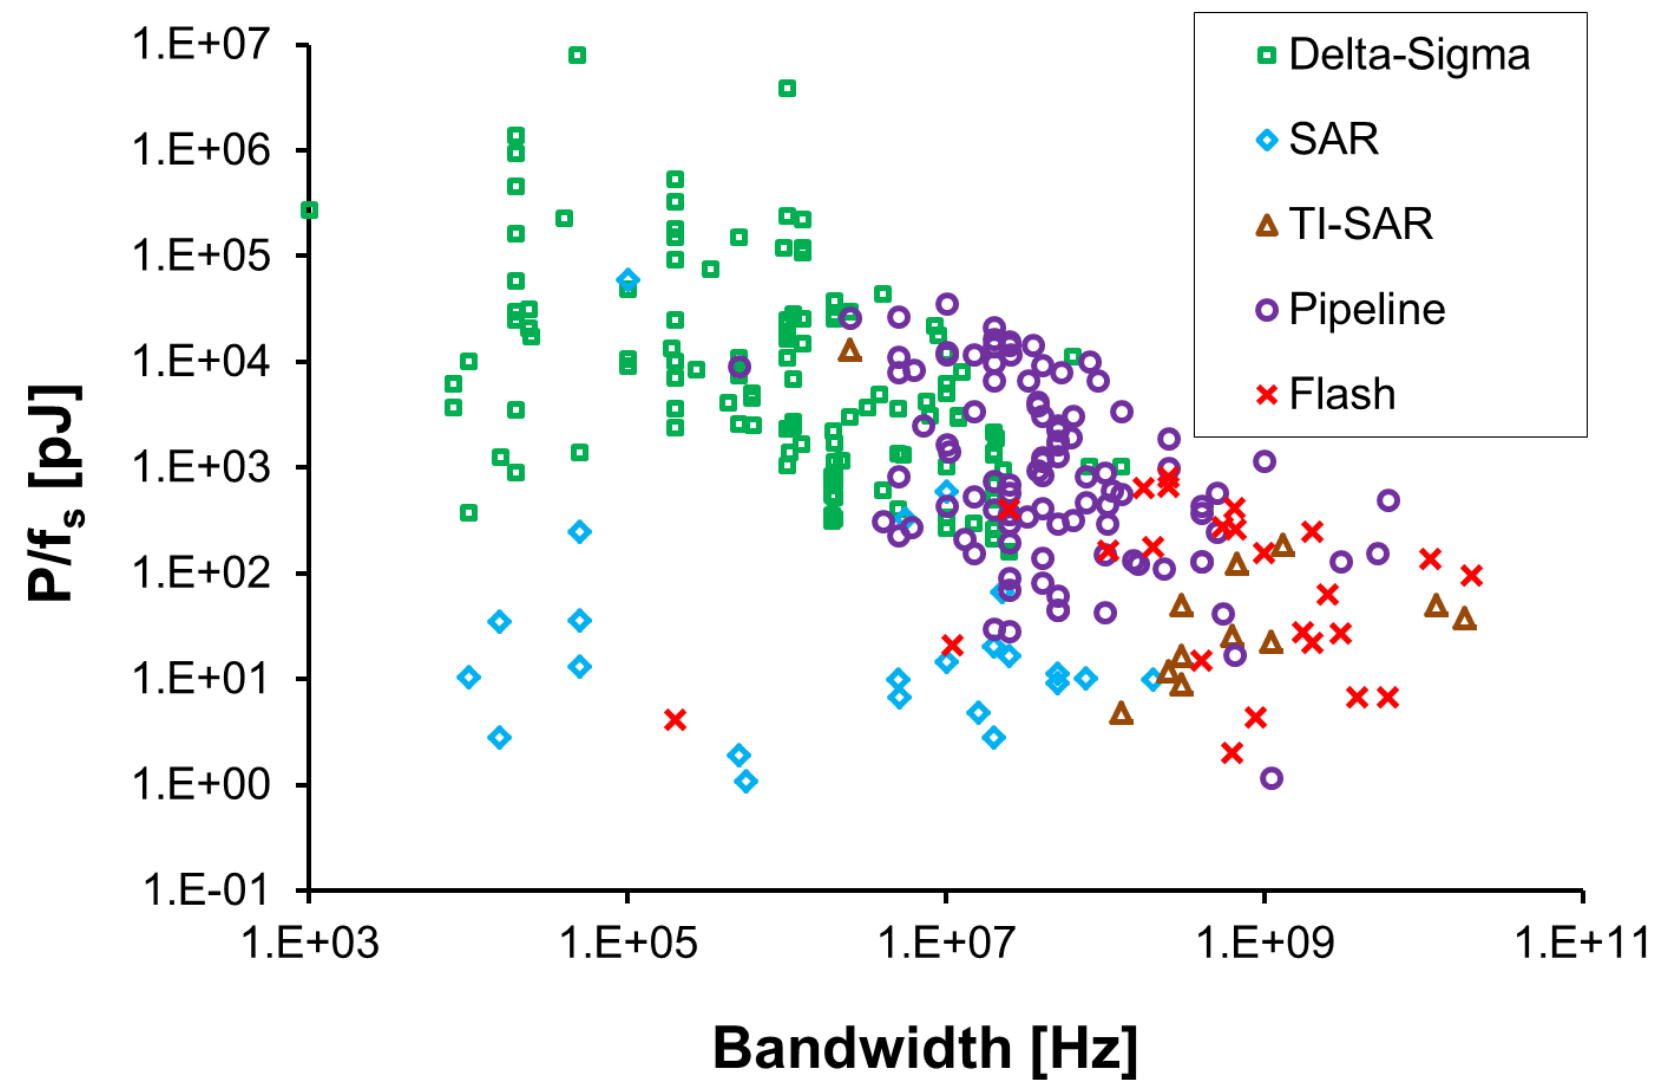
\includegraphics[height=2in]{figs/bw_vs_energy.png}
  \end{subfigure}
  \hfill
  \begin{subfigure}[t]{0.48\textwidth}
    \centering
    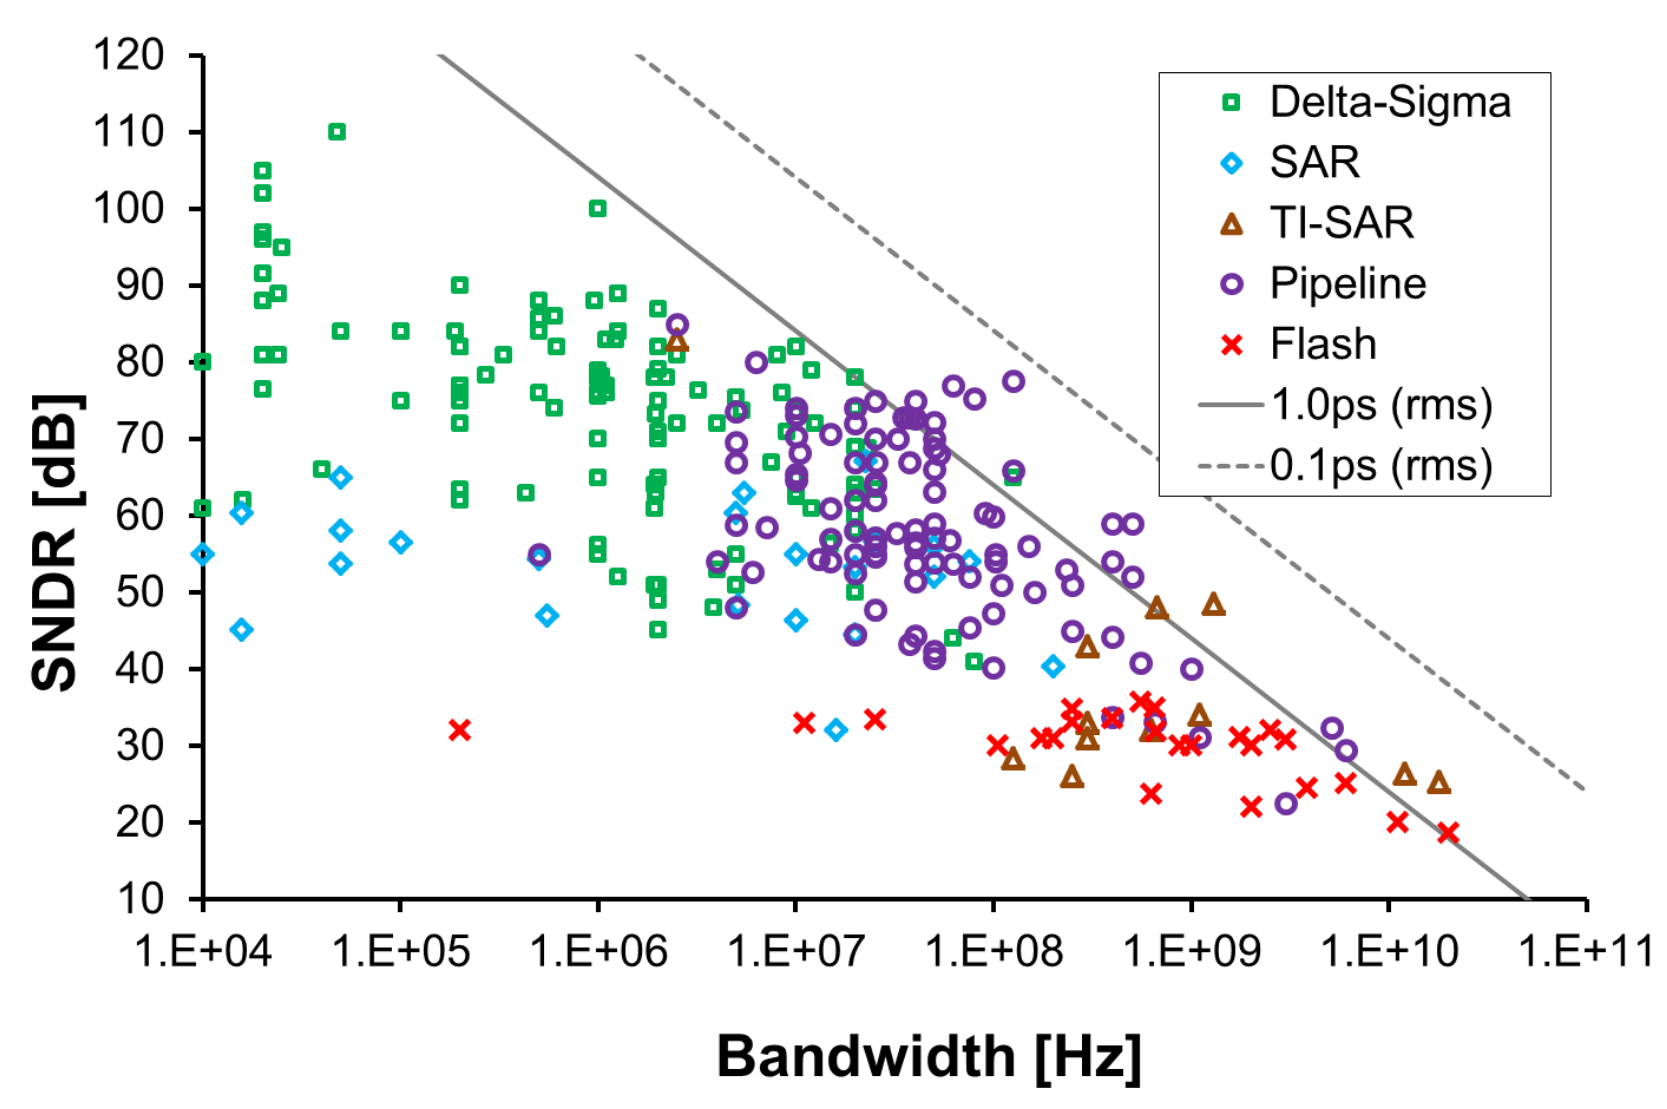
\includegraphics[height=2in]{figs/bw_vs_sndr.png}
  \end{subfigure}
  \caption{Plots from Murmann's (2012) ADC survey}
  \label{fig:adc_survey}
\end{figure}

Clearly a flash architecture cannot reasonably meet the SNDR requirement and would be more suitable for a higher bandwidth requirement.
The SAR architecture seems to deliver the best power efficiency, but it looks like the SOTA SAR ADCs cannot achieve a SNDR higher than 70 dB which makes achieving 65 dB a difficult proposition for this architecture.

The dynamic range spec translates to a 12-bit ADC, and scanning the table of ADC papers from Murmann's spreadsheet, either a pipeline or sigma-delta architecture seems appropriate.
% slide 32 lecture 9
According to figures from Pavan ("Understanding Delta-Sigma ADCs"), the sigma-delta ADC requires an oversampling ratio of 32-64 for a low-order modulator (2-3) and an OSR of 16-32 for a high-order modulator (4-6) to achieve SQNR above 65 dB.
This figure doesn't account for other noise sources from the SC stages used for error feedback, the sampling capacitor, or distortion.
This means the ADC has to run at $f_{adc} = 12.5 \cdot 2 \cdot \text{OSR}$ which is 400 - 800 MHz, imposing additional power requirements on the SAH stage to achieve settling time requirements.

In contrast the SAH and gain stages of the pipeline ADC can run at the Nyquist rate, and it should be able to achieve the SNDR spec.
I will design a model of a pipeline ADC.

\section{Pipeline ADC Analysis}
The dynamic range spec sets the number of bits for the ADC:
\begin{align*}
  \text{DR} &= (6.02 \cdot B) \text{ dB} \geq 70 \\
  B &\geq 11.6
\end{align*}

At least a 12-bit ADC is required to meet the dynamic range spec.
To determine each stage's optimal resolution and gain requires power and per-stage noise analysis first.

The bandwidth spec sets the sampling frequency of the pipeline ADC to at least $f_{samp} = 25$ MHz, and since the OTAs must settle the residue within half of the sample clock cycle this sets their required $g_m$.
This also places limits on the decision time of the flash ADC (within each stage) to 20ns.

The SNDR is determined by the quantization noise (from the selection of $B$), thermal noise from the SAH stage and every OTA gain stage, and distortion induced from non-linearities in the OTAs.

\subsection{Noise Analysis}
Consider the MDAC presented in lecture (Figure \ref{fig:mdac}) with 2 clock phases for sampling ($\phi_1$) and residual amplification ($\phi_2$).

\begin{figure}[h]
  \centering
  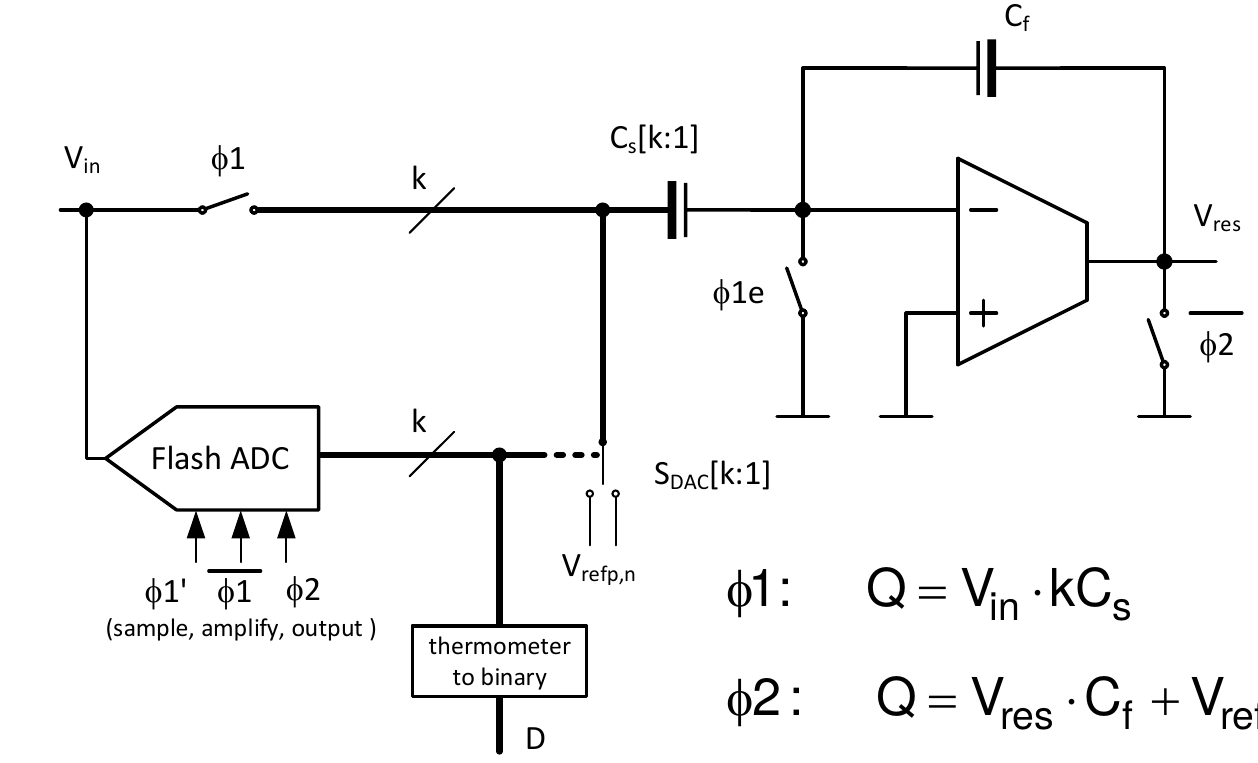
\includegraphics[width=0.6\textwidth]{figs/mdac.png}
  \caption{MDAC presented in lecture}
  \label{fig:mdac}
\end{figure}

\subsubsection{Sampling Phase}
During the first clock phase $\phi_1$, $V_{in}$ is sampled on $C_{s}$ and the switches $S_{\phi_1}$ and $S_{\phi_{1e}}$ inject voltage noise on $C_s$.
I'm not considering any noise injected due to charge injection caused by fast gating since bottom-plate sampling from $S_{\phi_{1e}}$ should alleviate this.

Both switches contribute thermal noise when they are on and the noise spectrum is shaped by $C_s$.
The total integrated noise across $C_s$ after sampling is:
\begin{align*}
  \overline{v^2_{samp}} = \frac{kT}{C_s}
\end{align*}

\subsubsection{MDAC Amplification Phase} % consider next stage loading
During the second clock phase $\phi_2$, the OTA develops $V_{res}$ by opening the $\phi_1$ switches and closing the switches to the DAC supply voltages.

\paragraph{OTA Noise}
Assume that the OTA is a simple 5 transistor circuit with one current source NMOS (M5), an NMOS input pair (M1/M2), and a PMOS active load (M3/M4).
The current noise of each transistor is $\overline{I^2_{n}} = 4kT\gamma g_m$.
\begin{align*}
  \overline{i^2_{out,n,inp}} &= 2 \cdot 4kT \gamma g_{m1} \\
  \overline{i^2_{out,n,mir}} &= 2 \cdot 4kT \gamma g_{m3} \\
  \overline{v^2_{out,n,tot}} &= \left(2 \cdot 4kT \gamma g_{m1} + 2 \cdot 4kT \gamma g_{m3} \right) \cdot (r_{o2} || r_{o4})^2 \\
  \overline{v^2_{in,n,tot}} &= \overline{v^2_{out,n,tot}} \cdot \frac{1}{g_{m1}^2 (r_{o2} || r_{o4})^2} = 2 \left( \frac{4kT\gamma}{g_{m1}} \right) + 2 \left( \frac{4kT\gamma g_{m3}}{g_{m1}^2} \right)
\end{align*}

\paragraph{OTA With Capacitive Feedback}
Now consider the OTA with $C_s$ connected to the (-) terminal, $C_f$ connected between the output and (-) terminal, and a load cap $C_L$ at the OTA's output representing the $C_s$ of the next stage.
\begin{align*}
  \beta (\text{FB factor}) &= \frac{C_f}{C_{s,k} + C_F} \\
  G_{CL} &= \frac{1}{\beta} \\
  C_{out,eff} &= C_L + (1 - \beta) C_f = C_{s,k+1} + (1 - \beta) C_f \\
  \omega_{p} &= \frac{\beta g_m}{C_{out,eff}} \\
  \overline{v^2_{n,ota,out}} &= \int_{0}^{\infty} \overline{v^2_{in,n,tot}} \frac{G}{1 + s / \omega_{p}} df \\
                             &= \overline{v^2_{in,n,tot}} \frac{\omega_p}{4} G^2 \\
                             &= \overline{v^2_{in,n,tot}} \frac{g_{m1}}{4 C_{out,eff} \beta^2}
\end{align*}

\paragraph{Total Thermal Noise}
The ADC consists of a sample and hold stage and N pipeline stages consisting of a flash ADC and MDAC.
\begin{align*}
  \overline{V^2_{n,in}} = \overline{v^2_{samp, 1}} + \overline{v^2_{n,ota,sah}} + \frac{\overline{v^2_{n,ota,1}} + \overline{v^2_{n,samp,2}}}{G_1^2} + \frac{\overline{v^2_{n,ota,2}} + \overline{v^2_{n,samp,3}}}{G_1^2 G_2^2} + \dots + \frac{\overline{v^2_{n,ota,N}}}{G_1^2 G_2^2 \dots G_N^2}
\end{align*}

\subsubsection{Quantization Noise}
The quantization noise power is:
\begin{align*}
  \overline{v^2_{n,quant}} = \frac{\Delta^2}{12} = \frac{{V_{DD} / 2^{12}}^2}{12} = 7.15 \text{ nV/Hz}
\end{align*}

\subsubsection{SNDR}
The SNDR captures quantization, thermal, and distortion induced noise.
\begin{align*}
  \text{SNDR} = \frac{P_{sig}}{P_{noise}} = \frac{(1.2 / \sqrt{2})^2}{\overline{v^2_{n,quant}} + \overline{v^2_{n,in}}}
\end{align*}

\subsection{OTA $g_m$} % how much OTA gain is needed to settle fast enough
The OTA needs to drive $V_{res}$ to the next stage's $C_s$.
The static error on $C_s$ should be under an LSB.

For an initial guess for $g_m$, I assume the OTA has a 1-pole transfer function and assume the settling to within 1 LSB must happen within 1 time constant.
\begin{align*}
  \tau &= \frac{C_{out,eff}}{\beta g_m} \\
       &= \frac{t_{settle}}{\ln (\text{1 LSB})} \\
       &= \frac{T_s / 2}{\ln (\text{1 LSB})}
\end{align*}

\subsection{Power Analysis} % translate gm to power (ignoring power of comparators and flash ADC)
The power consumption is dominated by the OTA.
The flash ADC, its comparators, and the switches consume relatively less power.
I'm neglecting the power required for the clock drivers and distribution.

\begin{align*}
  P = V_{DD} I_{d} = V_{DD} \left( \sum_{i=1}^{N} \frac{g_{m,i}}{\frac{g_{m,i}}{I_d}} \right)
\end{align*}

\subsection{Numbers}
For a first cut design, we will consider a 12-bit pipeline ADC built out of 12 1.5 bps stages to accomodate comparator offset varitions.
The noise of the ADC can be approximated as 

\section{Pipeline ADC Modeling}
The pipeline ADC is modeled in Python using separate classes for the flash ADC and the MDAC, then combining those into a stage and stages into a pipeline.

\end{document}
